\chapter{Ocena Sirius Web}

W tej pracy magisterskiej wykorzystano eksperymentalne i ciągle
rozwijane rozwiązanie \emph{Sirius Web}.
Mimo wykorzystywania tych samych metamodeli \gls{EMF} co dojrzała technologia
\emph{Sirius Desktop} występują pewne różnice. Zmiana platformy aplikacji z
natywnej na przeglądarkową również ma swoje zalety. W tym rozdziale technologia
\emph{Sirius Web} zostanie oceniona, a także porównana z jej poprzednikiem,
\emph{Sirius Desktop}, zarówno z perspektywy użytkownika edytora modeli, jak i
programisty tworzącego lub modyfikującego ten edytor.

\section{Interfejs użytkownika}

Interfejs użytkownika \emph{Sirius Web} przede wszystkim dostępny jest w
przeglądarce, która jest domyślnie zainstalowana
na większości komputerów konsumenckich. Nie jest wymagana instalacja dodatkowej
aplikacji natywnej jaką jest \emph{Sirius Desktop}, a później pobieranie
odpowiedniej definicji metamodelu. Osoba chcąca edytować diagram wystarczy, że
uruchomi stronę internetową i model zostanie jej wyświetlony lub będzie mogła
stworzyć nowy. Taka zmiana
znacznie ułatwia wdrożenie nowych osób do systemu i umożliwienie im~edytowania
lub~oglądania diagramów. Chcąc podzielić się z inną osobą modelem
wystarczy, że wysłany zostanie odpowiedni link, co jest dużo prostszą metodą
redukującą bariery związane z~przesyłaniem plików, które jest wymagane podczas
korzystania z \emph{Sirius Desktop}.

Sam interfejs użytkownika ma mniejsze możliwości dostosowywania przez
użytkownika. Układ
interfejsu jest sztywny, można co najwyżej zmienić szerokości lub wysokości
niektórych paneli albo je schować. Większe zmiany układu, jak zmiana kolejności
elementów, są~możliwe jedynie poprzez zmianę kodu źródłowego aplikacji
przeglądarkowej. Użytkownik nie~ma~na~nie~wpływu. Można natomiast na tyle
zmodyfikować kod interfejsu użytkownika, aby zrobić wszystko to, co jest
dostępne podczas dostosowywania interfejsu w \emph{Sirius Desktop}.

Domyślny układ edytora diagramów zdaje się być bardziej intuicyjny od tego w
\emph{Sirius Desktop}. Automatycznie rozwinięte są wszystkie potrzebne sekcje
--- drzewo obiektów modelu, informacje diagnostyczne, a także szczegóły
aktualnie zaznaczonego elementu modelu. W~\emph{Sirius Desktop} użytkownik
samemu musiał dostosować ten wygląd, co sprawia, że nowi użytkownicy mogli czuć
się bardziej zagubieni.

\subsection{Informacje diagnostyczne}

Zmianą na lepsze jest zwiększona częstość uruchamiania walidacji
modelu. W \emph{Sirius Web} informacje diagnostyczne pojawiają się po każdej
zmianie struktury modelu, podczas gdy~w~\emph{Sirius Desktop} należało
manualnie wywołać walidację modelu, aby zobaczyć zaktualizowane informacje.
Rozwiązanie z \emph{Sirius Web} pozwala użytkownikowi dużo szybciej dowiedzieć
się~o~problemach w modelu i je naprawić. Nie musi on także powtarzać w kółko
tej samej czynności walidacji.

Informacje diagnostyczne wyświetlane domyślnie w \emph{Sirius Web} to jedynie
błędy z walidacji składniowej modelu. Nie są uruchamiane reguły walidacji
semantycznej (\emph{Semantic Validation Rule}) zdefiniowane w metamodelu, co
zostało omówione w sekcji~\ref{sec:reguly-walidacyjne-metamodel}. Informacja
o~tym~problemie została zgłoszona w repozytorium projektu\footnote{
	\url{https://github.com/eclipse-sirius/sirius-components/issues/816}}.
Aby móc wykonywać walidację semantyczną modeli należy to rozwiązanie
zaimplementować samemu, co zostało zademonstrowane
w~sekcji~\ref{sec:walidacja-semantyczna-modelu}.
Oznacza to, że dodanie walidacji semantycznej do modelu jest znacznie
trudniejsze niż w \emph{Sirius Desktop}, ponieważ wymaga modyfikacji kodu
serwera aplikacyjnego. Ponadto, domyślnie nie ma przygotowanej architektury na
dodawanie reguł walidacji semantycznej, co~dodatkowo utrudnia ich wdrożenie.

Informacje diagnostyczne pojawiające się w \emph{Sirius Web} nie są
jawnie związane z konkretnymi elementami diagramu. Na diagramie nie widać
oznaczeń dla elementów, dla których występują błędy lub ostrzeżenia. Jedyna
informacja pozwalająca powiązać informację diagnostyczną z~konkretnym elementem
diagramu to nazwa tego elementu występująca w treści wiadomości diagnostycznej.
Jest to widoczne na rysunku~\ref{rys:validation-comparison-sirius-web}. Lepsze
rozwiązanie tego problemu występuje w
\emph{Sirius Desktop}, gdzie informacje diagnostyczne są ściśle powiązane z
konkretnym elementem diagramu, obok którego wyświetlona jest ikona błędu.
Wskazanie tej ikony powoduje wyświetlenie treści wiadomości diagnostycznej.
Jest to zaprezentowane na
rysunku~\ref{rys:validation-comparison-sirius-desktop}.
Takie rozwiązanie pozwala użytkownikowi szybciej zlokalizować niepoprawne
elementy diagramu i~zrozumieć co jest w nim błędnego. W \emph{Sirius Web}
użytkownik musi poświęcić więcej uwagi i~wysiłku w celu zlokalizowania
niepoprawnych elementów.

% \begin{noindent}
\begin{figure}
	\centering
	\begin{subfigure}{.49\textwidth}
		\centering
		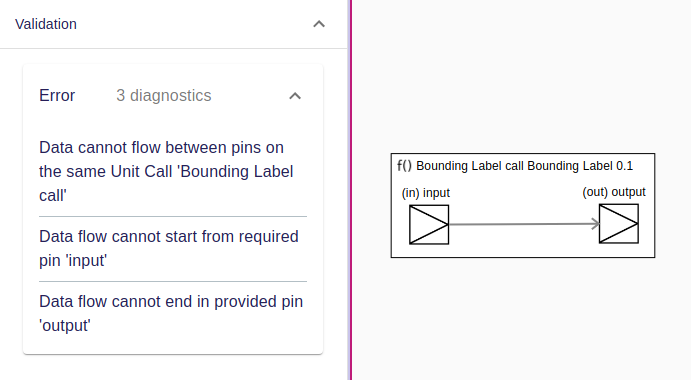
\includegraphics[width=.99\linewidth]{./images/sirius-web-semantic-validation-direction-and-no-loops-rules.png}
		\caption{Brak oznaczeń błędów na diagramie w \emph{Sirius
      Web}}\label{rys:validation-comparison-sirius-web}
	\end{subfigure}
  \begin{subfigure}{.49\textwidth}
		\centering
		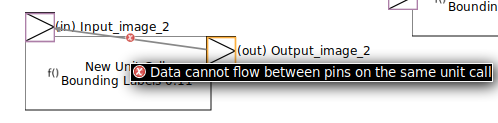
\includegraphics[width=.99\linewidth]{./images/sirius-desktop-example-semantic-validation-rule-failure.png}
		\caption{Oznaczenia błędów na diagramie w \emph{Sirius
      Desktop}}\label{rys:validation-comparison-sirius-desktop}
	\end{subfigure}

	\caption{Różnica w prezentacji informacji diagnostycznych}
\end{figure}
% \end{noindent}

\subsection{Narzędzia metamodelu EMF}

Innymi elementami zdefiniowanymi w metamodelu \gls{EMF}, które nie są w pełni
wspierane w \emph{Sirius Web}, są narzędzia edycji modelu. Podstawowe narzędzie
tworzenia nowego węzła w modelu działa poprawnie.
Pewne braki występują w większości pozostałych typów narzędzi. Narzędzie do
tworzenia krawędzi nie zwraca uwagi na zdefiniowane warunki określające możliwe
początki i końce połączenia (\emph{Connection Start Precondition} i
\emph{Connection Complete Precondition}). Użytkownik może stworzyć krawędź
między dwoma dowolnymi obiektami konkretnego typu i nie otrzymuje od edytora
wskazówek bazujących na semantyce modelu. Usterka została zgłoszona w
repozytorium projektu\footnote{
	\url{https://github.com/eclipse-sirius/sirius-components/issues/779}}.

Innym narzędziem związanym z krawędziami jest możliwość zmiany elementu
początkowego lub docelowego krawędzi w sposób wizualny poprzez zaznaczenie i
przesunięcie jednego z~końców krawędzi. W przypadku \emph{Sirius Web} taka
operacja jest niemożliwa, ponieważ krawędzie nie mają uchwytów na swoich
końcach. Takie uchwyty są dostępne w \emph{Sirius Desktop}, co~zostało pokazane
na rysunku~\ref{rys:sirius-desktop-reconnect-edge}. W wersji
przeglądarkowej tego edytora użytkownik może wybrać inny początek lub koniec
z listy elementów modelu, co jest rozwiązaniem podatnym na błędy i~wymagającym
większego wysiłku, albo usunąć istniejącą krawędź i stworzyć nową.
Usterka została zgłoszona w repozytorium projektu\footnote{
	\url{https://github.com/eclipse-sirius/sirius-components/issues/780}
}.

% \begin{noindent}
\begin{figure}[!hb]
  \centering

  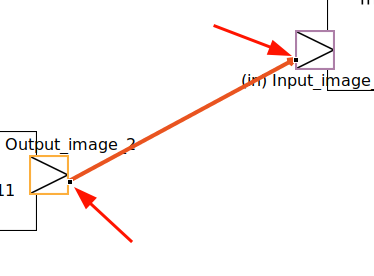
\includegraphics[width=0.5\linewidth]{./images/sirius-desktop-reconnect-edge.png}
  \caption{Uchwyty do zmiany końców krawędzi w \emph{Sirius
    Desktop}}\label{rys:sirius-desktop-reconnect-edge}
\end{figure}
% \end{noindent}

Kolejnym narzędziem metamodelu, które nie jest wspierane przez \emph{Sirius
	Web} są okna dialogowe pozwalające na wytworzenie bardziej
skomplikowanych
schematów edycji modelu czy~zautomatyzowanie niektórych czynności. Wyświetlenie
własnego okna dialogowego pozwalałoby na uproszczenie tworzenia nowego
wywołania modułu obliczeniowego w modelu, ponieważ użytkownik mógłby w oknie
dialogowym wskazać moduł obliczeniowy do wywołania. Takie narzędzie
przygotowano w \emph{Sirius Desktop}, co widać na
rysunku~\ref{rys:sirius-desktop-create-unit-call-dialog}. W \emph{Sirius
	Web} przy próbie wywołania tego narzędzia pojawia się błąd w konsoli
serwera
aplikacyjnego informujący, że to narzędzie nie jest zaimplementowane. Usterka
została zgłoszona w repozytorium projektu\footnote{
	\url{https://github.com/eclipse-sirius/sirius-components/issues/815}
}.

% \begin{noindent}
\begin{figure}[!hb]
  \centering

  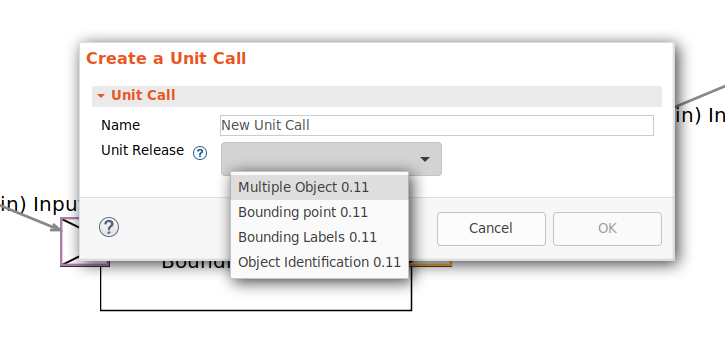
\includegraphics[width=0.95\linewidth]{./images/sirius-desktop-create-unit-call-dialog.png}
  \caption{Okno dialogowe w \emph{Sirius Desktop} ułatwiające tworzenie nowego
    obiektu}\label{rys:sirius-desktop-create-unit-call-dialog}
\end{figure}
% \end{noindent}

W \emph{Sirius Desktop} przybornik z narzędziami metamodelu jest wyświetlony
w osobnym oknie, co widać po prawej stronie
rysunku~\ref{rys:sirius-desktop-model-editor-tools-right}. Zawiera on w każdym
momencie wszystkie dostępne narzędzia.
Użytkownik musi nauczyć się które narzędzia są dostępne dla których obiektów
modelu i kiedy mogą zostać wykorzystane. Przykładowo, po wybraniu narzędzia
\emph{Data Flow} służącego do tworzenia połączeń między portami użytkownik może
wskazać jedynie jeden z~portów. Brakuje wskazówek co należy dalej zrobić.
\emph{Sirius Web} inaczej reprezentuje narzędzia. Są one umieszczone w
przyborniku pokazywanym po kliknięciu myszą na element diagramu. Wyświetlone są
jedynie narzędzia związane z wybranym elementem, co upraszcza wybór, ponieważ
użytkownik nie musi wiedzieć które narzędzia mają sens dla wybranego elementu
--- \emph{Sirius Web} automatycznie ogranicza wybór. Jest to rozwiązanie lepsze
niż w \emph{Sirius Desktop} pod względem intuicyjności interfejsu.

% \begin{noindent}
\begin{figure}[!hb]
  \centering

  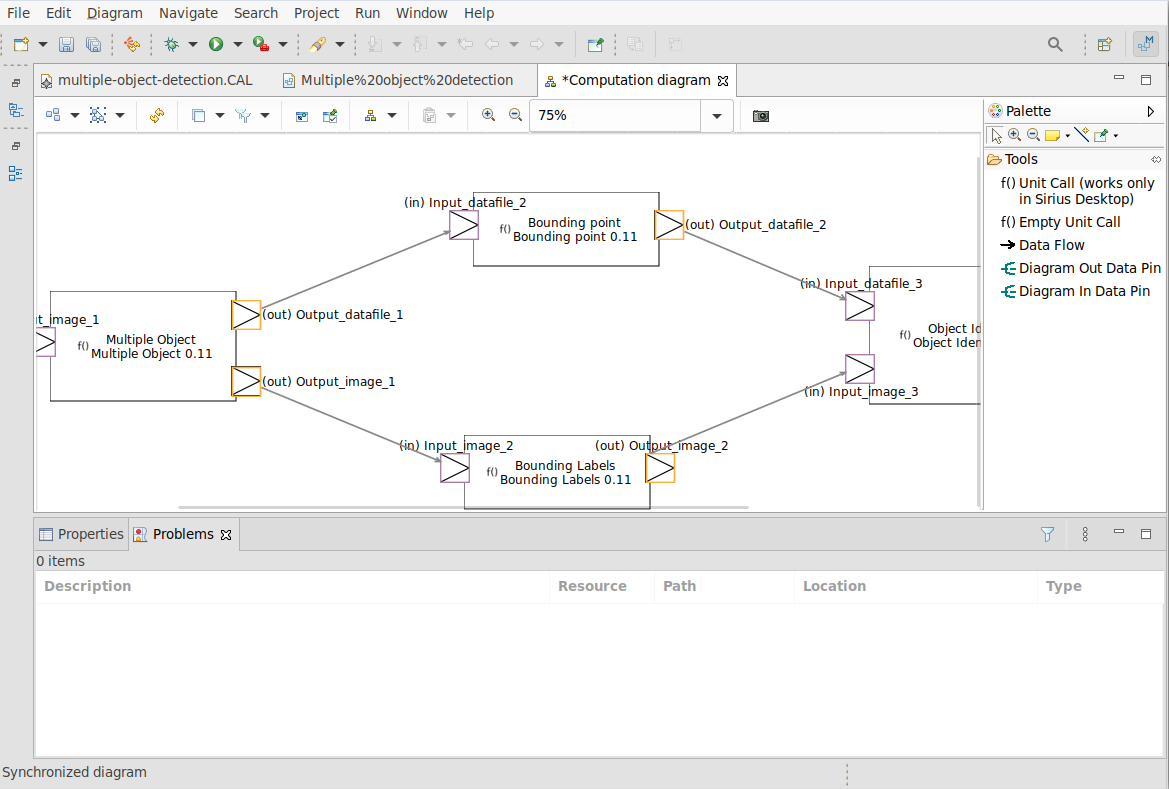
\includegraphics[width=0.95\linewidth]{./images/sirius-desktop-model-editor.png}
  \caption{Interfejs \emph{Sirius Desktop} z narzędziami po prawej
    stronie}\label{rys:sirius-desktop-model-editor-tools-right}
\end{figure}
% \end{noindent}

W \emph{Sirius Web} występują 2 problemy związane z przybornikiem narzędzi. Po
pierwsze, niektóre narzędzia są wyświetlane podwójnie. Można to zobaczyć na
rysunku~\ref{rys:sirius-web-duplicate-tools}. Pokazane są dwie ikony ze
strzałką służące tworzeniu połączenia wychodzącego z portu \emph{output}, a
także dwie ikony związane z usunięciem elementu (\emph{DeleteComputedDataPin}
oraz ikona kosza). Taka duplikacja może zaskoczyć użytkownika i sprawić, że nie
będzie on wiedział który przycisk należy wybrać, aby zrealizować oczekiwany cel
oraz jakie są różnice między tymi przyciskami. W rzeczywistości oba przyciski w
obu przypadkach mają taki sam skutek, więc duplikacja jest niepotrzebna.

% \begin{noindent}
\begin{figure}[!ht]
  \centering

  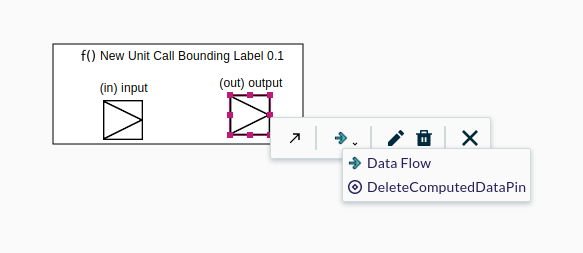
\includegraphics[width=0.95\linewidth]{./images/sirius-web-duplicate-tools.png}
  \caption{Zduplikowane narzędzia w \emph{Sirius
    Web}}\label{rys:sirius-web-duplicate-tools}
\end{figure}
% \end{noindent}

Kontynuując temat przybornika w \emph{Sirius Web}, z
rysunku~\ref{rys:sirius-web-duplicate-tools} wynika, że dla portu wywołania
modułu obliczeniowego dostępne są dwa narzędzia usuwające go. W
metamodelu rzeczywiście jest takie narzędzie, ale jest ono tam wyłącznie po to,
aby zabronić usuwania tych elementów z~diagramu, ponieważ są one zarządzane
automatycznie i ich usunięcie natychmiast sprawiłoby, że diagram stałby
się niepoprawny semantycznie (wywołanie modułu obliczeniowego miałoby mniej
portów niż powiązany z nim moduł obliczeniowy). W \emph{Sirius Desktop}
usunięcie tego portu z diagramu jest niemożliwe, co widać na
rysunku~\ref{rys:sirius-desktop-blocked-deleting-pins}.
\emph{Sirius Web} wyświetla odpowiednie ikony i~pozwala je wybrać, co skutkuje
wyświeleniem błędu w konsoli serwera aplikacyjnego, a~po kilku sekundach
wyświetleniem niejasnej wiadomości o przekroczeniu czasu przetwarzania żądania,
przedstawionego na rysunku~\ref{rys:sirius-web-timeout-when-deleting-pins}.
Takie rozwiązanie jest mylące dla użytkownika i pogarsza wrażenia z
wykorzystania edytora.

% \begin{noindent}
\begin{figure}[!hb]
  \centering

  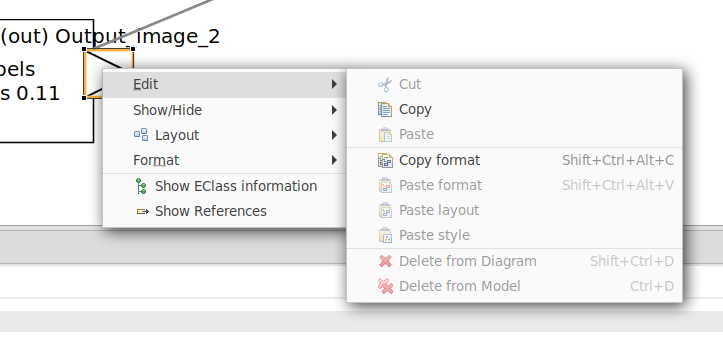
\includegraphics[width=0.95\linewidth]{./images/sirius-desktop-blocked-deleting-pins.png}
  \caption{Zablokowana możliwość usunięcia portu wywołania modułu
    obliczeniowego w \emph{Sirius Desktop}}\label{rys:sirius-desktop-blocked-deleting-pins}
\end{figure}
% \end{noindent}

% \begin{noindent}
\begin{figure}[!hb]
  \centering

  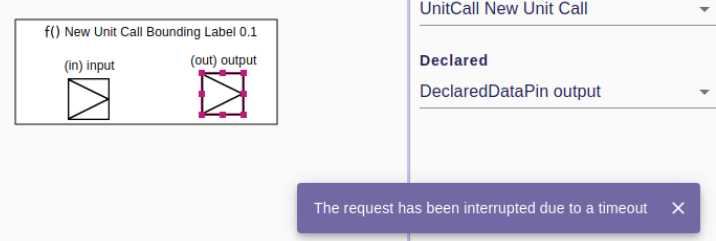
\includegraphics[width=0.95\linewidth]{./images/sirius-web-timeout-when-deleting-pins.png}
  \caption{Błąd podczas próby usunięcia portu wywołania modułu obliczeniowego w
    \emph{Sirius Web}}\label{rys:sirius-web-timeout-when-deleting-pins}
\end{figure}
% \end{noindent}

\subsection{Właściwości tylko do odczytu}

\emph{Sirius Web} niepoprawnie obsługuje właściwości elementów modelu oznaczone
jako
\emph{tylko do~odczytu} (\emph{readonly}). Czasami takie właściwości można
swobodnie zmieniać, a czasami podczas zmiany pojawia się błąd w konsoli serwera
aplikacyjnego i właściwość nie jest zmieniona. Oba zachowania są niepoprawne,
ponieważ oczekiwaniem dla takich właściwości jest, że będą one tylko do
odczytu, a więc w interfejsie użytkownika nie będzie można wybrać dla nich
innej wartości. W \emph{Sirius Desktop} użytkownik nie może zmienić wartości
tych właściwości, ale tylko w jednej z dwóch zakładek pozwalających na
wyświetlenie detali obiektu. Druga zakładka pozwala na ich zmianę.
Zgłoszono w tym temacie dwie usterki w repozytorium
projektu \emph{Sirius Web}\footnote{
	\url{https://github.com/eclipse-sirius/sirius-components/issues/813}
}\textsuperscript{,}\footnote{
	\url{https://github.com/eclipse-sirius/sirius-components/issues/814}
}. Jako obejście problemu w tej pracy magisterskiej zrezygnowano z~używania
właściwości \emph{tylko do odczytu}.

\subsection{Wyświetlanie elementów diagramu}

Niektóre elementy na diagramie wyświetlane są w inny sposób. Porty, które w
metamodelu zostały oznaczone jako węzły krawędziowe (\emph{Border Node}), w
\emph{Sirius Desktop} rzeczywiście są~wyświetlane na krawędzi swojego rodzica
(węzła wywołania modułu obliczeniowego), natomiast w \emph{Sirius Web} są
wyświetlane w jego środku. Usterka jest znana i została zgłoszona\footnote{
	\url{https://github.com/eclipse-sirius/sirius-components/issues/956}
}. Różnice w wyświetlaniu węzłów krawędziowych zostały zaprezentowane na
rysunku~\ref{rys:border-node-difference}.
Przy okazji warto zauważyć, że \emph{Sirius Web} nie obsługuje wyświetlania
krawędzi węzłów krawędziowych. Te widoczne na
rysunku~\ref{rys:border-node-sirius-web} pochodzą z ikony i zostały specjalnie
dodane po odkryciu tej usterki. Została ona zgłoszna w repozytorium
projektu\footnote{
	\url{https://github.com/eclipse-sirius/sirius-components/issues/783}}.

% \begin{noindent}
\begin{figure}
	\centering
	\begin{subfigure}{.49\textwidth}
		\centering
		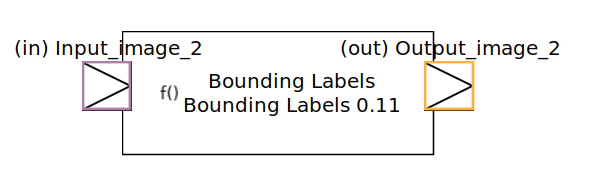
\includegraphics[width=.99\linewidth]{./images/border-node-sirius-desktop.png}
		\caption{Węzły krawędziowe w \emph{Sirius Desktop} są wyświetlane na
      krawędzi}
	\end{subfigure}
	\begin{subfigure}{.49\textwidth}
		\centering
		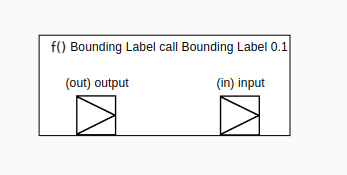
\includegraphics[width=.99\linewidth]{./images/border-node-sirius-web.png}
		\caption{Węzły krawędziowe w \emph{Sirius Web} są wyświetlane wewnątrz
      węzła}\label{rys:border-node-sirius-web}
	\end{subfigure}

    \caption{Różnica w wyświetlaniu węzłów
      krawędziowych}\label{rys:border-node-difference}
\end{figure}
% \end{noindent}

Ikony obiektów metamodelu również są wyświetlane inaczej niż w \emph{Sirius
	Desktop}. Jeżeli rozmiar ikony przekracza 16 pikseli na 16 pikseli,
ikona
zaczyna nachodzić na etykietę obiektu. Porównanie zachowania obu edytorów w
tym przypadku zostało przedstawione na
rysunku~\ref{rys:sirius-multiline-labels}. Problem został zgłoszony w
repozytorium projektu\footnote{
	\url{https://github.com/eclipse-sirius/sirius-components/issues/782}
}. Jako próba jego obejścia zmniejszono ikony do rozmiaru 16 na 16 pikseli, aby
tekst był czytelny.

% \begin{noindent}
\begin{figure}
	\centering
	\begin{subfigure}{.49\textwidth}
		\centering
    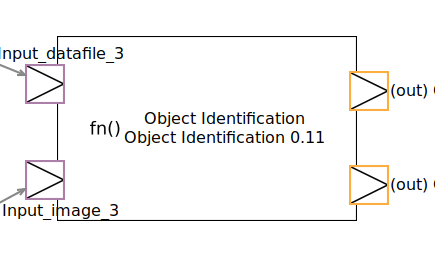
\includegraphics[width=.8\linewidth]{./images/sirius-desktop-multiline-label.png}
		\caption{Dwuwierszowa etykieta obiektu w \emph{Sirius Desktop}}
    \vspace{20pt}
	\end{subfigure}
	\begin{subfigure}{.49\textwidth}
		\centering
		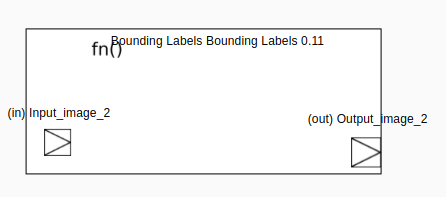
\includegraphics[width=.99\linewidth]{./images/sirius-web-multiline-label.png}
		\caption{Ta sama etykieta w \emph{Sirius Web}}\label{rys:border-node-sirius-web}
    \medskip
    {\footnotesize Ponadto, ikona o rozmiarze większym niż $16\times16$ pikseli nachodzi na tekst.}
	\end{subfigure}

    \caption{Wyświetlanie dwuwierszowych
      etykiet oraz większych ikon}\label{rys:sirius-multiline-labels}
\end{figure}
% \end{noindent}

Pozostając w temacie etykiet obiektów, są z nimi 2 problemy. Po pierwsze,
znaki nowej linii w etykietach są zamieniane na zwykłe odstępy. Widać to na
rysunku~\ref{rys:sirius-multiline-labels}, gdzie w \emph{Sirius Desktop} nazwa
wywoływanego modułu
obliczeniowego znajduje się w nowej linii, natomiast w \emph{Sirius Web} cała
etykieta to jedna linia. Zaburza to estetykę diagramu. Usterka została
zgłoszona w~repozytorium projektu\footnote{
	\url{https://github.com/eclipse-sirius/sirius-components/issues/781}
}. Drugim z problemów związanym z etykietą jest jej~edycja w sytuacji, gdy
etykieta jest obliczana w języku \gls{AQL} na podstawie kilku właściwości
obiektu. \emph{Sirius Desktop} nie pozwala na bezpośrednią edycję całej
etykiety w tym przypadku, a \emph{Sirius Web} wyświetla pole do zmiany tekstu
tylko po to, aby go później zignorować --- po zatwierdzeniu zmiany etykieta
wraca do swojej początkowej wartości, a w konsoli serwera aplikacyjnego
wyświetlany jest błąd. Usterka została zgłoszona w repozytorium
projektu\footnote{
	\url{https://github.com/eclipse-sirius/sirius-components/issues/784}
}.

Warunkowe zmiany stylu elementów modelu (\emph{Style Customizations}) działają
poprawnie. Dzięki nim ikony portów w \emph{Sirius Web} zmieniają się na
podstawie swoich parametrów (krotności danych i tokenów). Drugi ze styli
warunkowych w metamodelu dotyczący zmiany koloru krawędzi portu ze względu na
jego typ (wejściowy lub wyjściowy) nie może zostać zweryfikowany, ponieważ
krawędzie te w ogóle nie są wyświetlane.

\emph{Sirius Web} nie wprowadza niektórych ograniczeń, które są przestrzegane w
\emph{Sirius Desktop}. Jednym z nich jest zablokowanie możliwości zmiany
rozmiaru węzłów. W metamodelu zabroniono zmiany rozmiaru portów i takiego
zachowania można się spodziewać w aplikacji natywnej, natomiast w \emph{Sirius
	Web} zmiana ich rozmiaru jest możliwa bez ograniczeń, co zostało
przedstawione na
rysunku~\ref{rys:change-node-size}. Problem został zgłoszony w repozytorium
projektu\footnote{
	\url{https://github.com/eclipse-sirius/sirius-components/issues/785}}.

% \begin{noindent}
\begin{figure}[!hb]
  \centering

  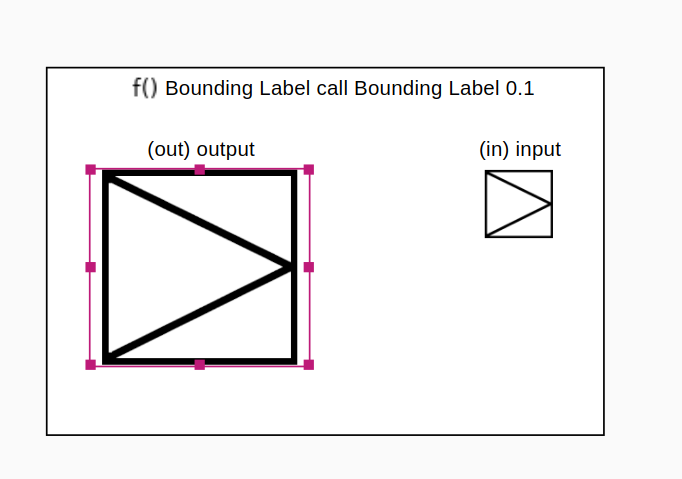
\includegraphics[width=0.6\linewidth]{./images/change-node-size.png}
  \caption{Zmieniony rozmiar węzłów w Sirius Web}\label{rys:change-node-size}
\end{figure}
% \end{noindent}

\subsection{Wydajność}

Interfejs użytkownika \emph{Sirius Web} zazwyczaj reguje na zmiany natychmiast.
Animacje używane w edytorze diagramów występujące podczas dodawania lub
usuwania z niego elementów sprawiają, że aplikacja jest przyjemniejsza w użyciu
i sprawia wrażenie bardziej dopracowanej, a~jednocześnie pomaga zrozumieć co
się dzieje w modelu. Jest to szczególnie ważne, gdy~zmiany są wykonywane przez
inną osobę edytującą ten diagram w czasie rzeczywistym.
Problem z wydajnością występuje podczas przesuwania elementów w \emph{Sirius
	Web}. Interfejs przesuwa elementy z opóźnieniem, a po upuszczeniu
elementów
często ignoruje przyciśnięcia klawiszy myszy przez około sekundę. Jest to
wyjątek pośród ogólnie płynnego interfejsu, co~dodatkowo uwidacznia ten
problem.

Udostępnienie aplikacji do edycji diagramów w przeglądarce powoduje, że na
jej wydajność wpływa szybkość łącza Internet użytkownika. Architektura
rozwiązania \emph{Sirius Web} powoduje, że aplikacja często musi komunikować
się z serwerem aplikacyjnym. Dzieje się tak z uwagi na fakt, że informacje o
modelu przechowywane są w bazie danych, a metamodel \gls{EMF} jest
interpretowany przez serwer. Do przeglądarki komunikowane są jedynie informacje
o~modelu, a nie metamodel. Dla przykładu, wywołanie narzędzia tworzącego nowe
wywołanie modułu obliczeniowego wymaga przesłania zapytania typu
\emph{mutation} do serwera aplikacyjnego, otrzymania odpowiedzi potwierdzającej
tą zmianę, po czym asynchronicznie serwer wysyła jeszcze 3 wiadomości
za pomocą połączenia \emph{GraphQL} \emph{subscription}:

\begin{itemize}
	\item \texttt{diagramEvent} z nową zawartością diagramu,
	\item \texttt{validationEvent} z nowym zestawem informacji
	      diagnostycznych,
	\item \texttt{treeEvent} z nową zawartością drzewa modelu.
\end{itemize}

Te 3 wiadomości zawierają informacje o \textbf{całym} modelu. W przeciwieństwie
do podejścia przyrostowego, w którym przesyłane byłyby jedynie informacje o
zmianach względem poprzedniego stanu modelu, podejście z przesyłaniem
wszystkich informacji za każdym razem powoduje, że przez sieć przesyłanych jest
znacznie więcej danych. Ponadto, aplikacja przeglądarkowa musi je
zinterpretować i odpowiednio zaaplikować w interfejsie, co również wymaga
większej ilości obliczeń. Znaczenie tego problemu jest proporcjonalne do
wielkości modelu --- im większy model, tym więcej informacji jest przesyłanych
przez sieć przy każdej jego modyfikacji.

Aplikacja działała płynnie podczas korzystania z niej w sytuacji, w której
serwer aplikacyjny był uruchomiony na komputerze, na którym wykonywano test.
Opóźnienia wynikające z narzutu na przesyłanie danych przez sieć były
zauważalne, gdy została sztucznie ograniczona szybkość połączenia internetowego
za pomocą narzędzi programisty w przeglądace \emph{Google Chrome}.
Używanie ustawienia \emph{Fast 3G}, które ogranicza szybkość pobierania danych
do 1.5~Mb/s i opóźnieniu
500~ms~\cite{network-throttling-profiles-stackoverflow} sprawiło, że aplikacja
przestała być używalna z uwagi na długi czas pobierania danych o modelu.
Szczegółowe czasy oczekiwania na wyświetlenie elementów interfejsu z włączonym
sztucznym opóźnieniem zostały zaprezentowane w
tabeli~\ref{tab:sirius-web-ui-delay-throttled}.

\begin{table}[!b]
	\centering
	\begin{tabular}{p{5cm}c}
		\toprule
		Element interfejsu       & Czas oczekiwania (sekundy) \\
		\midrule
		Drzewo obiektów modelu   & 92                         \\
		Informacje diagnostyczne & 92                         \\
		Diagram                  & 154                        \\
		\bottomrule
	\end{tabular}
	\caption{Czas oczekiwania na wyświetlenie elementów interfejsu
		\emph{Sirius
			Web} z włączonym sztucznym opóźnieniem \emph{Fast
			3G}}\label{tab:sirius-web-ui-delay-throttled}
\end{table}

Opóźnienie sieciowe nie ma wpływu na modyfikację pozycji elementów. Użytkownik
może płynnie przesuwać węzły na diagramie. Wszelkie inne operacje wymagają
informacji z serwera aplikacyjnego. Oznacza to, że korzystanie z edytora
\emph{Sirius Web} wymaga szybkiego i stabilnego połączenia sieciowego. Nie jest
to wymagane w przypadku \emph{Sirius Desktop}, w którym wydajność zależy
wyłącznie od szybkości komputera używanego do edycji modeli.

Możliwym rozwiązaniem problemu przesyłania zbyt dużej ilości danych przez sieć
w~\emph{Sirius Web} byłoby zmiana zawartości przesyłanych wiadomości na
podejście przyrostowe. Komunikaty zawierałyby jedynie informacje o zmianach,
które zazwyczaj można wyrazić zwięźlej niż~przesyłając cała zawartość
zaktualizowanego modelu.

\section{Problemy techniczne}

Poza problemami możliwymi do zauważenia w interfejsie użytkownika \emph{Sirius
	Web} pojawiły się~też~problemy widzialne głównie dla inżynierów
pracujących nad edytorem diagramów.

Największym problemem rozwiązania \emph{Sirius Web} jest brak możliwości
uwierzytelniania połączenia \emph{GraphQL} \emph{subscription} obsługiwanego za
pomocą technologii \emph{WebSocket}. Za~pomocą tego połączenia przesyłane są
informacje o zawartości modeli i szczegółach wszystkich ich~elementów. Jeżeli
\emph{Sirius Web} zostałby wykorzystany do edycji modeli z danymi wrażliwymi
lub poufnymi, nie byłoby gwarancji, że osoby postronne lub nieautoryzowane
nie~mają do nich dostępu. Jest to spora wada, która może zdyskwalifikować
\emph{Sirius Web} jako rozwiązanie do~edycji diagramów w niektórych
zastosowaniach. Usterka ta została zgłoszona w repozytorium
projektu\footnote{
	\url{https://github.com/eclipse-sirius/sirius-components/issues/846}}.

Podczas korzystania z \emph{Sirius Web} widoczne były błędy w konsoli serwera
aplikacyjnego po~wykonaniu pewnych operacji. W przypadku wywołania narzędzia
metamodelu odpowiedzialnego za kaskadowe usunięcie kilku elementów na raz, z
których niektóre mogą nie~istnieć, wyświetlany był wyjątek
\texttt{NullPointerException} pomimo, że w tej samej sytuacji \emph{Sirius
	Desktop} zachowywał się poprawnie i nie informował o występujących
błędach.
Usterka została zgłoszona w repozytorium projektu\footnote{
	\url{https://github.com/eclipse-sirius/sirius-components/issues/791}
}. Obejściem problemu było dodanie bloków \texttt{If}~w~metamodelu
sprawdzającego czy odpowieednia właściwość jest ustawiona (ma wartość inną niż
\texttt{null}) zanim element zostanie usunięty.

Kolejny wydruk na konsolę, który zdarzał się po wywołaniu narzędzia metamodelu
do~kaskadowego usuwania elementów, jest informacja o wiszącej referencji do
elementu, który nie znajduje się w modelu (wyjątek
\texttt{DanglingHREFException}). Jest to błąd, który pojawiał się wyłącznie w
\emph{Sirius Web} --- w \emph{Sirius Desktop} nie było problemów z kaskadowym
usuwaniem elementów. Usterka została zgłoszona w repozytorium
projektu\footnote{
	\url{https://github.com/eclipse-sirius/sirius-components/issues/792}
}.

Niektóre z usterek zgłoszonych w repozytorium projektu na platformie
\emph{GitHub} zostały naprawione podczas pisania tej pracy magisterskiej.
Dodane zostało wsparcie dla akcji metamodelu wywołujących kod w języku Java
(\emph{External Java Action})\footnote{
	\url{https://github.com/eclipse-sirius/sirius-components/issues/613}}.
Naprawiony został także błąd polegający na niepoprawnym obliczaniu ścieżek do
ikon elementów w stylach warunkowych\footnote{
	\url{https://github.com/eclipse-sirius/sirius-components/issues/865}
}. Dzięki temu można było wykorzystać język \gls{AQL} do dynamicznego
ustalenia ścieżki, co pozwoliło na uniknięcie tworzenia 7 zbliżonych do
siebie styli warunkowych.

Innym problemem pojawiającym się z nieokreśloną częstością jest wyjątek
\texttt{NonNullable\-FieldWasNullException} występujący podczas
dodawania wielu
elementów na~raz~do~modelu. Taka sytuacja dzieje się, gdy do diagramu zostaje
dodane nowe wywołanie modułu obliczeniowego. Może wtedy być stworzonych wiele
obiektów podczas obsługi jednego zapytania \emph{GraphQL}. Wystąpienie tego
wyjątku uniemożliwia dalszą pracę z modelem, ponieważ w interfejsie użytkownika
nie zostaje wyświetlony żaden element diagramu. Nie pomaga odświeżenie strony
internetowej czy ponowne uruchomienie serwera aplikacyjnego. Pracę można
kontynuować tworząc nowy model i licząc na to, że problem nie wystąpi ponownie,
lub~usuwając z modelu wszystkie elementy pojedynczo, korzystając z drzewa
elementów modelu. Usterka została zgłoszona w repozytorium
projektu\footnote{
	\url{https://github.com/eclipse-sirius/sirius-components/issues/828}
}. Jest to kolejny poważny problem, który uniemożliwia komfortową pracę z
edytorem diagramów, a niedeterminizm jego występowania sprawia, że jest on
trudny w zdiagnozowaniu. Nie pojawia się~on~w~przypadku tworzenia elementów
pojedynczo. Możliwym rozwiązaniem byłaby zmiana podejścia tworzenia wielu
elementów na raz na wysyłanie wielu zapytań \emph{GraphQL} dodającym po jednym
elemencie zamiast jednego zapytania dodającego kilka elementów. Jest to
natomiast rozwiązanie mniej wydajne i bardziej komplikujące kod aplikacji.

Niedogodnością pojawiającą się podczas pracy z aplikacją przeglądarkową
\emph{Sirius Web} jest fakt, że nazwy komponentów w dostarczonym kodzie
JavaScript są zobfuskowane. Utrudnia to analizę struktury aplikacji w
narzędziach programisty w przeglądarce. Zrzut ekranu prezentujący zobfuskowane
nazwy komponentów pochodzące z biblioteki \texttt{sirius-components} jest
widoczny na rysunku~\ref{rys:sirius-web-minified-component-names}. Problem
został zgłoszny w repozytorium
projektu\footnote{
	\url{https://github.com/eclipse-sirius/sirius-components/issues/831}
}.

% \begin{noindent}
\begin{figure}[!hb]
  \centering

  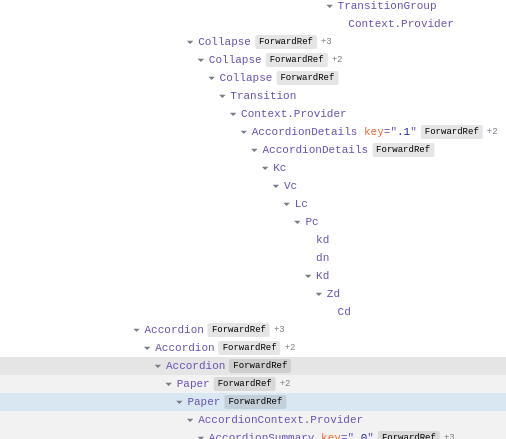
\includegraphics[width=0.7\linewidth]{./images/sirius-web-minified-component-names.png}
  \caption{Zobfuskowane nazwy komponentów z biblioteki
    \texttt{sirius-components}}\label{rys:sirius-web-minified-component-names}
\end{figure}
% \end{noindent}

\section{Użycie własnego metamodelu}

\emph{Sirius Web} jest technologią eksperymentalną i nie posiada ona jeszcze
swojej dokumentacji technicznej. Oznacza to, że zrozumienie jak ona działa i co
należy zmienić, aby osiągnąć zamierzone rezultaty wymaga analizy kodu
źródłowego, inżynierii wstecznej, a~także metody prób i~błędów podczas
dokonywania zmian w
kodzie. Dostępne jest jedynie repozytorium \texttt{sirius-web} służące jako
przykład wykorzystania biblioteki z repozytorium \texttt{sirius-components}
do zbudowania edytora diagramów.
Pomocnym okazała się możliwość zadawania pytań autorom projektu poprzez
tworzenie zgłoszeń na platformie \emph{GitHub}. Właśnie w ten sposób zadano
pytanie z prośbą o wyjaśnienie jak można użyć własnego metamodelu \gls{EMF} w
\emph{Sirius Web}\footnote{
	\url{https://github.com/eclipse-sirius/sirius-web/issues/36}
}. W odpowiedzi otrzymano krótkie wyjaśnienie oraz listę miejsc w kodzie
wymagających edycji.

Instrukcja ta była pomocna, ale dla osób nie mających wcześniej styczności z
technologią \gls{EMF} i metamodelami tworzonymi w niej okazała się
niewystarczająca, ponieważ wymagane były dodatkowe zasoby wyjaśniające jak taki
metamodel stworzyć~\cite{dokumentacja-sirius-desktop,dokumentacja-aql} oraz jak
umożliwić wykorzystanie pakietów Javy wygenerowanych przez \gls{EMF} w systemie
\emph{Maven}~\cite{maven-tycho-tutorial}.
Duża liczba nowych technologii do wykorzystania i skonfigurowania wymagała
metody prób i błędów, która w połączeniu z długim czasem kompilacji aplikacji
(zazwyczaj około jednej minuty) powodowała frustrację. Z pewnością pomocne
byłoby
stworzenie dokumentacji opisującej krok po kroku proces tworzenia własnego
metamodelu i wykorzystania go w \emph{Sirius Web}. Taka instrukcja obniżyłaby
barierę wejścia i sprawiłaby, że rozpoczęcie pracy z tą technologią byłoby dużo
szybsze i przyjemniejsze.

Zaskoczeniem było też odkrywanie kolejnych funkcjonalności metamodelu
\gls{EMF}, które nie były obsługiwane przez \emph{Sirius Web}, lub były
obsługiwane wyłącznie częściowo. Zespół rozwijający tą technologię wykorzystuje
ciągle ten sam metamodel podczas swojej pracy, który nie korzysta ze
wszystkich możliwości \gls{EMF}. Konsekwencją tego jest brak ekspozycji autorów
\emph{Sirius Web} na różne problemy wynikające z braku kompatybilności i
konieczność powiadamiania ich o usterkach za pomocą \emph{GitHub Issues}.
Pomocne w tym przypadku byłoby udostępnienie przez autorów projektu listy
funkcjonalności metamodeli \gls{EMF}, które są wspierane, a także wypisanie
tych, które są nieobsługiwane. W ten sposób przygotowując własny edytor
na~bazie
\emph{Sirius Web} można byłoby od razu zorientować się z których narzędzi można
swobodnie korzystać, a na które nie warto zużywać czasu w metamodelu \gls{EMF}
bo wiadomo, że należy je~opracować samemu.

Podsumowując, znając wszystkie kroki potrzebne do wykorzystania własnego
metamodelu \gls{EMF} w \emph{Sirius Web} można tego dokonać w krótkim czasie.
Wymagane sa zmiany jedynie kilku miejsc w kodzie aplikacji. Brakuje
dokumentacji tej technologii, która wskazałaby kolejne kroki tego
procesu, aby rozpoczęcie pracy było prostsze, szybsze i mniej frustrujące.

\section{Dodawanie funkcjonalności do edytora}

Podstawowy edytor diagramów dostępny w repozytorium \texttt{sirius-web}
pozwala na edycję modeli w sposób podobny do \emph{Sirius Desktop}.
Jego kod źródłowy jest natomiast prostszy w edycji i rozszerzeniu w porównaniu
do kodu \emph{Sirius Desktop}. Pozwala to dostosować edytor do swoich potrzeb i
dodać funkcjonalności, które pomogą użytkownikom szybciej lub prościej pracować
z modelami, lub których brakuje w porównaniu do natywnej wersji edytora.

Modyfikacja kodu źródłowego serwera aplikacyjnego zazwyczaj sprowadza się do
dodania nowych klas i modyfikacji niewielkiego fragmentu kodu, aby były one
używane, chociaż nie~jest to wymagane w każdym przypadku. Dzieje się tak dzięki
funkcjonalności wstrzykiwania zależności (\emph{Dependency Injection})
technologii \emph{Java Spring}. Tak właśnie było w przypadku dodawania nowych
mutacji \emph{GraphQL}, aby dodać możliwość tworzenia modułu obliczeniowego
wraz z jego wywołaniem w obrębie jednej transakcji. Trzeba było wtedy
dodać kilka klas odpowiedzialnych za serializację i deserializację danych, oraz
klasy odpowiedzialne za~przetwarzanie zapytania, a później \emph{Sirius Web}
automatycznie wykrył je i dodał możliwość wysyłania tego rodzaju mutacji.
Jest to bardzo wygodne rozwiązanie, ponieważ kod można łatwo rozszerzyć bez
modyfikacji istniejących klas w znacznym stopniu, co jest zgodne z~zasadą
\emph{Open--Closed Principle} % chktex 8
z akronimu \emph{SOLID}. Mówi ona, że klasy powinny być otwarte
na~rozszerzenie, ale zamknięte na modyfikację.

Nietrudno było również dodać mechanizm odpowiedzialny za walidację semantyczną
metamodelu. Wymagało to modyfikacji istniejącej klasy związanej z przesyłaniem
informacji diagnostycznych, ale modyfikacja ta była w dużej części dodaniem
nowego kodu.

W obu przypadkach zmiany okazały się proste do wykonania, jednak z uwagi na
brak dokumentacji technicznej \emph{Sirius Web} należało spędzić dodatkowy czas
na znalezienie odpowiedniego miejsca w kodzie do modyfikacji. Często wymagało
to zajrzenia do kodu źródłowego z repozytorium \texttt{sirius-components}, w
którym znajduje się większość kodu biblioteki edytora, i zastosowaniu tam
inżynierii wstecznej. W ten sposób ustalano jakie interfejsy należy
zaimplementować, aby dostarczyć nowych funkcjonalności w serwerze aplikacyjnym
lub~edytorze. Udostępnienie dokumentacji technicznej \emph{Sirius Web} dla osób
rozwijających edytor i umieszczenie przykładów takich rozszerzeń znacznie
przyśpieszyłoby pracę z edytorem i~sprawiłoby, że praca z nim byłaby
przyjemniejsza.

Część dodawanych funkcjonalności edytora wymaga zmodyfikowania kodu źródłowego
aplikacji przeglądarkowej \emph{Sirius Web}. Zmiany te mają różny rozmiar i
poziom skomplikowania w zależności od miejsca umieszczenia
dodawanych lub zmienianych elementów interfejsu.
Nowe podstrony aplikacji wyświetlające całkiem nowy układ interfejsu są proste
do zaimplementowania, podobnie jak modyfikacja elementów niezwiązanych
bezpośrednio z modelami. Wynika to~z~faktu, że istniejące elementy interfejsu
aplikacji \emph{Sirius Web} to komponenty biblioteki \emph{React} pochodzące z
repozytorium \texttt{sirius-components}, które nie umożliwiają zmiany wyglądu
lub~dodawania nowych elementów w swoim wnętrzu.

Standardowym, choć nieco uciążliwym rozwiązaniem w tym przypadku, jest
skopiowanie do~własnego rozwiązania kodu komponentów wyższego poziomu
składających
się z mniejszych
części, a następnie dodanie lub zmodyfikowanie ich układu. Takim złożonym
komponentem wyższego poziomu jest \texttt{Workbench} omówiony w
sekcji~\ref{sec:wyswietlenie-zawartosci-przybornika-w-sirius-web} wyświetlający
cały interfejs edytora diagramów wraz z panelami po prawej i lewej stronie.
Oprócz wyświetlania komponentów zawiera on także logikę synchronizującą
wyświetlany interfejs,
która również musiała być~skopiowana, ponieważ nie została udostępniona osobno
z repozytorium \texttt{sirius-components}. Podobnie z niektórymi komponentami
niższego poziomu wykorzystywanymi przez \texttt{Workbench} --- je także trzeba
było skopiować, aby zachować ten sam wygląd interfejsu użytkownika.

Ostatecznie dla widoku edytora diagramów kod skopiowany z repozytorium
\texttt{sirius-\allowbreak components} % chktex 1
stanowi ponad $37\%$ całego kodu
odpowiedzialnego za ten widok (1245 z 3320 linii). Jest to kod, który musi być
utrzymywany przez osoby przygotowujące edytor, co utrudnia utrzymanie projektu.
Zwiększa on także czas jego kompilacji, ponieważ jest on kompilowany jako
część aplikacji mimo, że w rzeczywistości pochodzi z biblioteki. W niektórych
przypadkach zwiększa on ilość danych przesyłanych do przeglądarki, ponieważ kod
ten musi być przez nią przetworzony, co negatywnie wpływa na szybkość ładowania
aplikacji. Wszystkich tych negatywnych efektów można byłoby uniknąć, gdyby z
\texttt{sirius-components} udostępnionych było więcej komponentów i funkcji.

Dzięki lepszym narzędziom wspomagającym inspekcję kodu biblioteki
\texttt{sirius-components} znalezienie odpowiedniego miejsca do modyfikacji
kodu aplikacji przeglądarkowej jest prostsze niż było to w przypadku serwera
aplikacyjnego \emph{Sirius Web}. Nadal wymagało to jednak inżynierii wstecznej
i czytania kodu źródłowego komponentów. Dodanie dokumentacji technicznej
opisującej dostępne do wykorzystania komponenty oraz ich parametry umożliwiłoby
szybsze zapoznanie się z biblioteką i wykorzystanie jej. Największym problemem
do rozwiązania w~przypadku komponentów z biblioteki \texttt{sirius-components}
jest udostępnienie możliwości modyfikowania interfejsu użytkownika
bez konieczności kopiowania dużych fragmentów kodu.

\section{Aktualizacja wersji edytora}

Projekt \emph{Sirius Web} jest aktywnie rozwijany. Od 15 grudnia 2021 r.\ do 15
stycznia 2022~r.\ zostało wprowadzone do niego 45 zmian\footnote{
	\url{https://github.com/eclipse-sirius/sirius-components/pulse/monthly}
}, w których zmieniono sumarycznie ponad 9~tysięcy linii kodu.
Nowe wersje zawierające poprawki usterek lub nowe funkcjonalności są~wydawane
co miesiąc. Każda nowa wersja wymaga serii zmian, które muszą być wykonane
w~kodzie źródłowym aplikacji przeglądarkowej lub serwera aplikacyjnego
\emph{Sirius Web}, ponieważ kod~\texttt{sirius-components} zmienia się w sposób
niezachowujący wstecznej kompatybilności~\cite{sirius-components-changelog}.

Aktualizacja do nowej wersji edytora wymaga wprowadzenia zmian w kodzie
źródłowym \emph{Sirius Web}, które zostały wykonane przez zespół pracujący nad
projektem w repozytorium \texttt{sirius-web}. Dzięki używaniu narzędzia
\emph{git} zmiany te mogą być wprowadzone automatycznie za pomocą kilku komend
linii poleceń. Wprowadzanie zmian w repozytorium \texttt{sirius-web} pokazuje
jak one powinny być wykonane, co jest znacznym ułatwieniem w porównaniu
do~wyłącznego czytania listy zmian nowego wydania biblioteki.

Każda modyfikacja kodu \emph{Sirius Web} powoduje, że jest to potencjalne
miejsce na wystąpienie konfliktów podczas aplikowania zmian za pomocą narzędzia
\emph{git}, które zostały wprowadzone w~nowszej wersji edytora.
Dzieje się tak, ponieważ kod w naszej wersji edytora zaczyna się wtedy różnić
od edytora z repozytorium \texttt{sirius-web} i narzędzie \emph{git} nie może
wywnioskować jak ma rozwiązać te niekompatybilności.
Im większe zmiany, tym większa szansa na konflikt i tym jest on trudniejszy w
rozwiązaniu.
W niektórych przypadkach zmiany w~\texttt{sirius-web} nie~wynikają ze złamania
kompatybilności wstecznej, a z nowych funkcjonalności edytora. Często
wymagają one wtedy większego wysiłku we wdrożeniu do naszej kopii edytora.
W takich chwilach można się zastanowić czy nie łatwiej byłoby zignorować tą
zmianę wprowadzoną w~\emph{Sirius Web}, ponieważ rozwiązywanie konfliktów w
kodzie jest zbyt czasochłonne.

Największym problemem utrzymania aplikacji \emph{Sirius Web} jest utrzymanie
kodu źródłowego komponentów aplikacji przeglądarkowej skopiowanych z
repozytorium \texttt{sirius-components}. Ich definicja znajduje się w innym
repozytorium, więc narzędzie \emph{git} nie wykryje automatycznie tych zmian.
Należy więc manualnie śledzić zmiany dla skopiowanych komponentów i samemu
wprowadzać je do kodu. Jest to podejście znacznie bardziej czasochłonne
niż to wykorzystujące automatyczną konsolidację zmian narzędzia \emph{git}.
Pominięcie wprowadzenia zmian w tych komponentach może spowodować błędy podczas
działania aplikacji, ponieważ może zostać naruszony kontrakt między tymi
komponentami a resztą kodu.

Podsumowując, aktualizacja edytora do nowszej wersji zazwyczaj jest prosta, ale
wymaga tym więcej czasu, im bardziej go zmodyfikowaliśmy w porównaniu do
oryginalnej wersji z~repozytorium \texttt{sirius-web}. We wprowadzaniu zmian
znacznie pomaga narzędzie \emph{git}. Każda nowa wersja biblioteki
\texttt{sirius-components} do tej pory zawierała zmiany łamiące kompatybilność
wsteczną, co warto wziąć pod uwagę planując proces aktualizacji.
